\documentclass{article}
\usepackage{enumitem}
\usepackage{graphicx}
\usepackage{grffile}
\usepackage{float}
\begin{document}
\title{%
 Deliverable 1\\
 \large An identification of problems, derivation of high level requirements\\
 \large and an articulation of features using controlled notation
}
\author{Epic Group}
\date{}
\maketitle

\section*{Introduction}
The purpose of this report is to identify and express high level requirements
regarding a potential software system via structured notation. We will express
the contents of our report in the following format.
\begin{enumerate}
\item \textbf{Problem Statements}: A series of problem statements which will
investigate a number of problems we will solve via our software prototype.
\item \textbf{User Stories}: An idenfitication of features based on the problem
statement previously specified.
\item \textbf{Low-Fidelity Prototype}: A paper physical sketch of the UI 
elements integrated with a storyboard-like chronological script.
\item \textbf{High-Fidelity Prototype}: A computerised render of the
low-fidelity prototype previously specified.
\end{enumerate}
Our report will strictly harbor to controlled software engineering notation, 
such as the utilisation of user stories and Connextra notation.
\section{Problem Statements}
We will enumerate over a series of problem statements, tangibly solved by
software, potentially resolved in our prototype. Subsequently, we will choose
to target a specific problem statement within the remainder of our report.
\subsection{Problem Statement}
Recommendations of visual media on contemporary popular internet platforms are
inaccurate, biased or limited. Recommendation algorithms on such platforms are
often a small subsection of a larger media streaming or distribution service, 
restricting the scope of recommendation to those within such a service. Moreover, 
recommendation systems are typically implemented with small data sets and cheap 
computational cost as a priority. As a result, recommendations provided to a 
user are fragmented, unreliable and erroneous.
\subsection{Problem Statement}
Information presented by news media outlets and online sources of information
can frequently be misleading or malicious. In addition, the advent of social
media platforms permitting and stimulating the concept of sudden, mass 
popularity has encouraged the threat of misinformation spreading routinely and
to great negitive effect. In response, the employment of paid moderators have
only further exacerbated the issue, with themselves enforcing their baiases
regarding which information is legal.
\subsection{Problem Statement}
Due to the prevalence of database leaks combined with the tendency of internet
users to share credentials across multiple platforms, identities on the internet
are frequently hijacked. Moreover, specific individuals are often targeted in
order to spread disinformation and aid in monentary theft. Current database
credential storage technologies are inadquate in reducing user harm during the
seemingly inevitable event that a webserver security solution is bypassed.

\section{User Stories}
\begin{table}[h]
\begin{tabular}{|l|}
\hline
\textbf{Feature:} Search movie by key words   \\
\textbf{As a:} User\\
\textbf{So that:} I can find the movie I want\\
\textbf{I want to:} Search movie by its key words\\
\textbf{Scenario:} Search movie by key words\\
\textbf{GIVEN:} I am on sysName home page\\
\textbf{WHEN:} I type key words into "Search Movie" search bar\\
\textbf{AND:} I press "search" button\\
\textbf{THEN:} I should see all movies which are related to the key words\\
\hline
\end{tabular}
\end{table}

\begin{table}[h]
\begin{tabular}{|l|}
\hline
\textbf{Feature:} \\
\textbf{As a:} \\
\textbf{So that:} \\
\textbf{I want to:} \\
\textbf{Scenario:} \\
\textbf{GIVEN:} \\
\textbf{WHEN:} \\
\textbf{THEN:} \\
\hline
\end{tabular}
\end{table}

\section{Low-Fiedelity Prototype}
The following images are rough sketches of a potential final website design.
\subsection{Landing Page}
\begin{figure}[H]
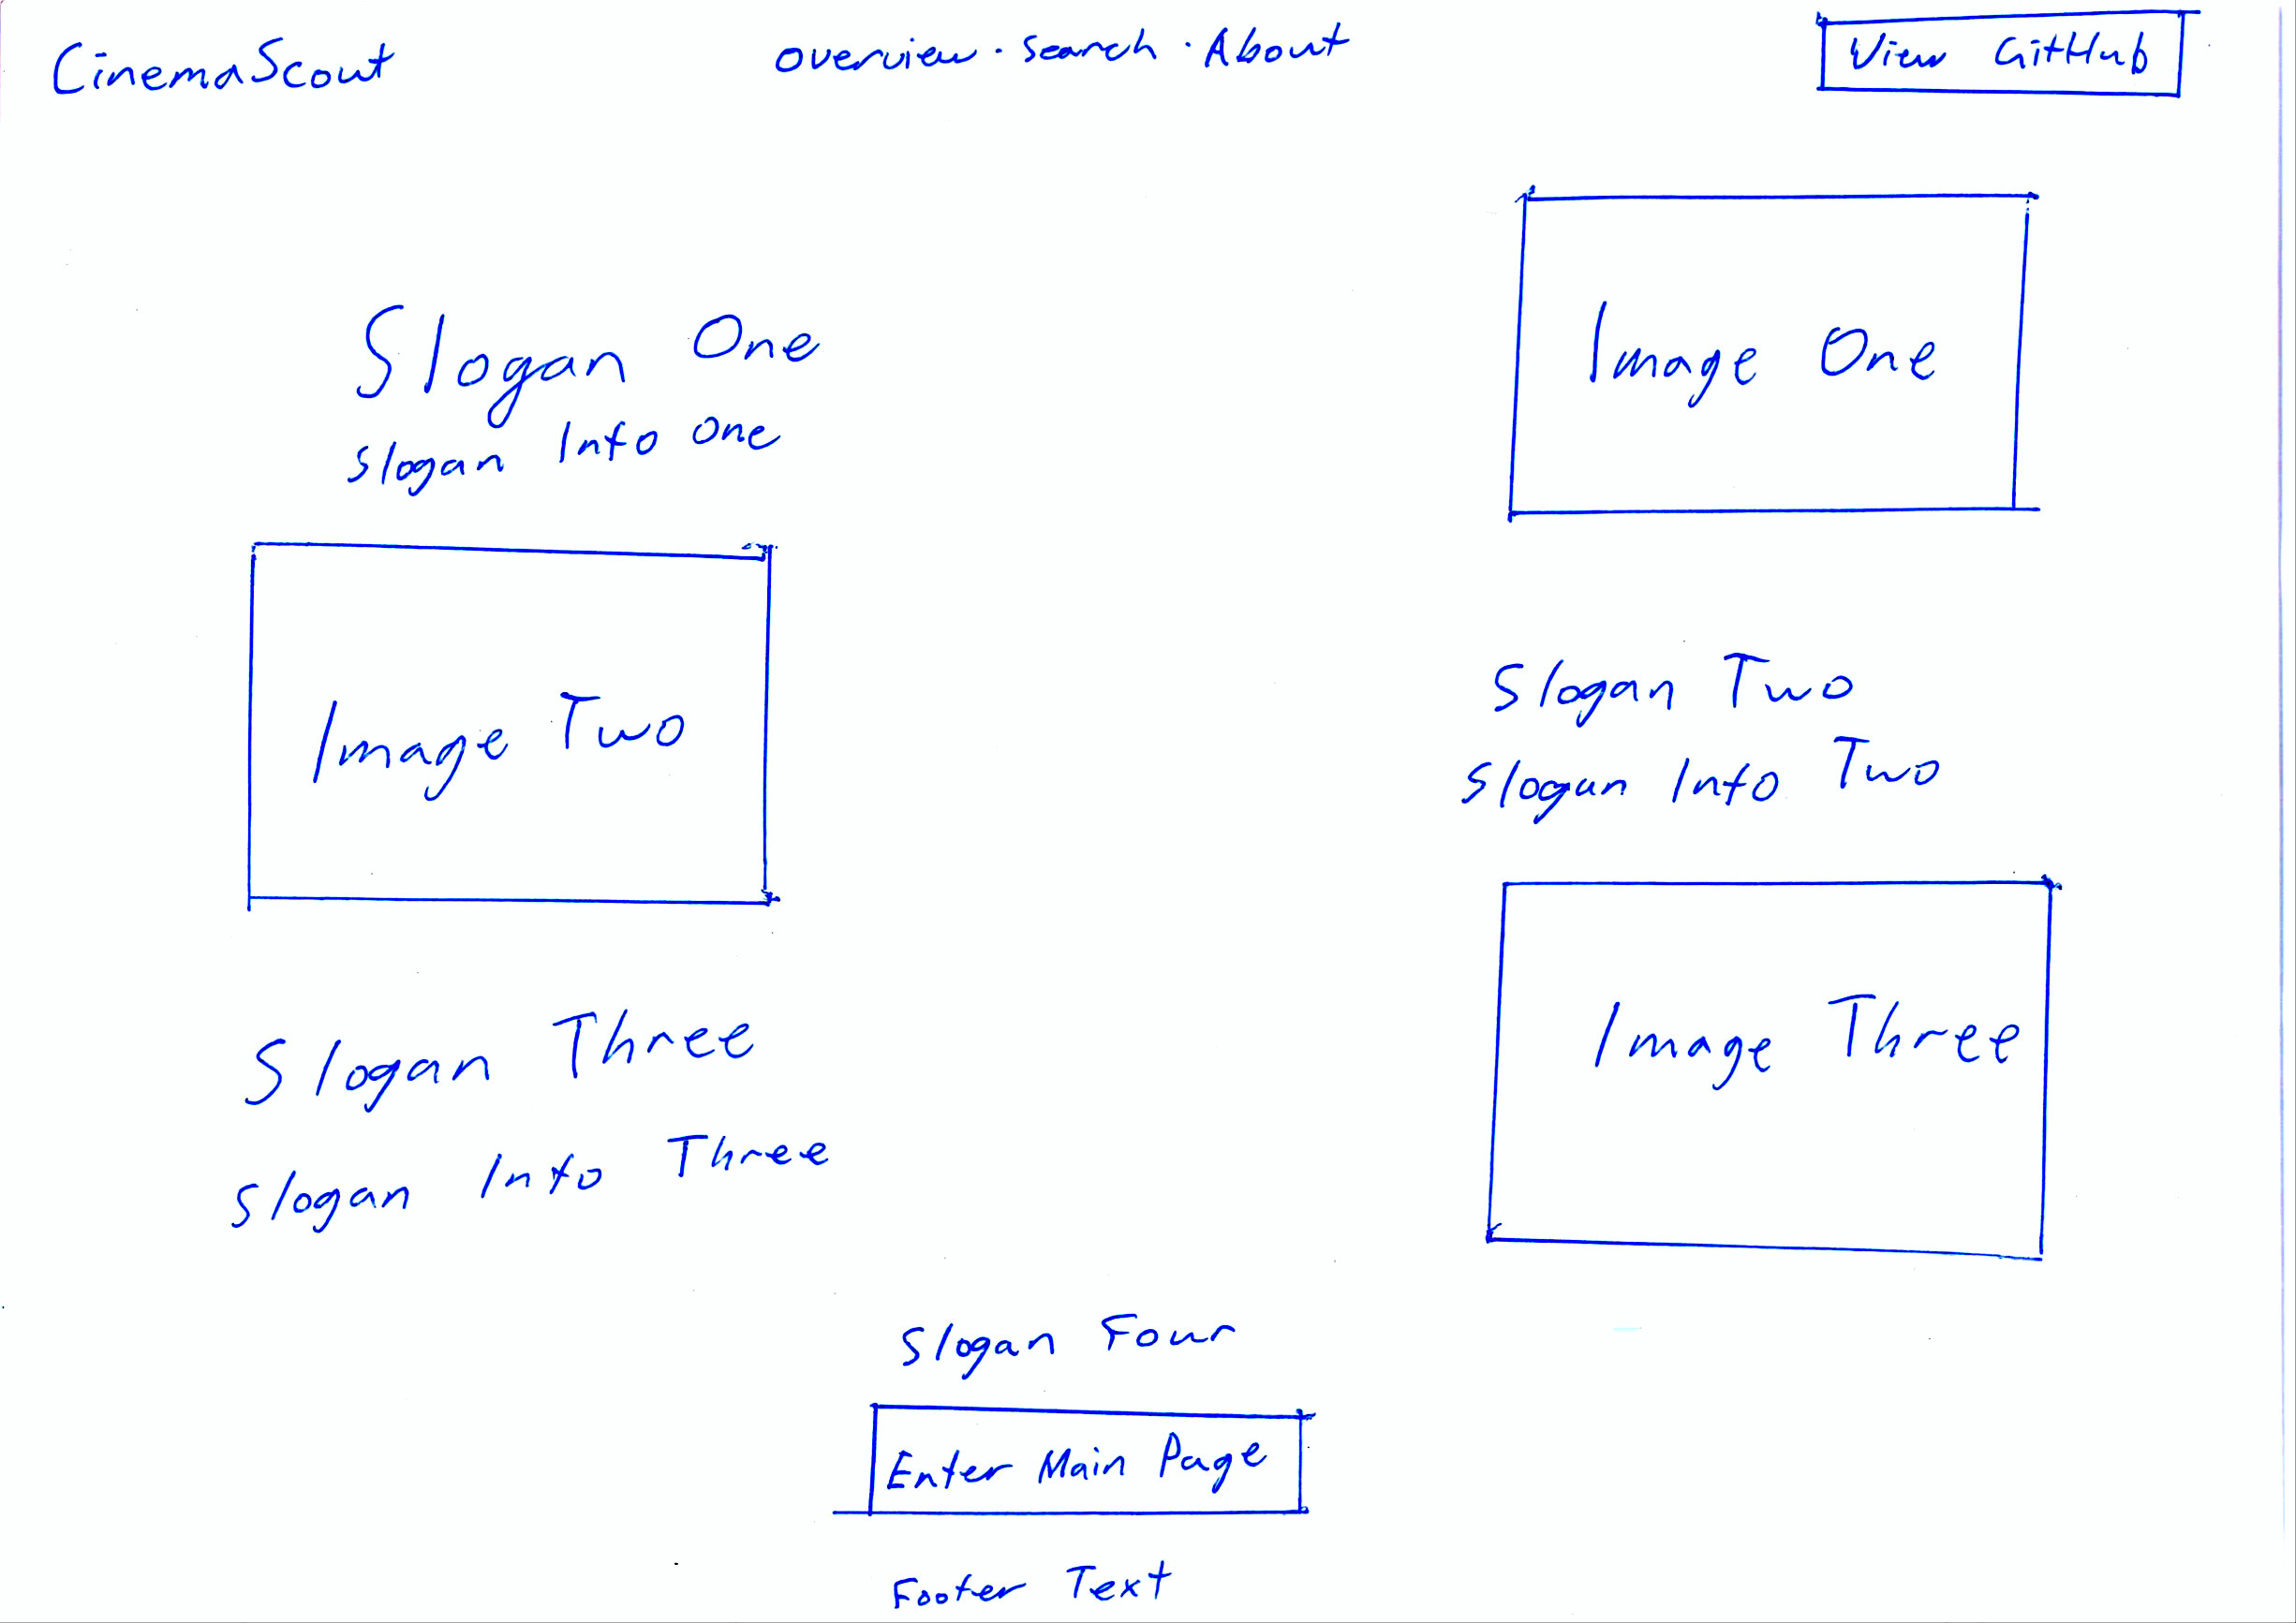
\includegraphics[width=\columnwidth]{res/landing.jpg}
\caption{Rough sketch of the landing page.}
\end{figure}
\subsection{Search Page}
\begin{figure}[H]
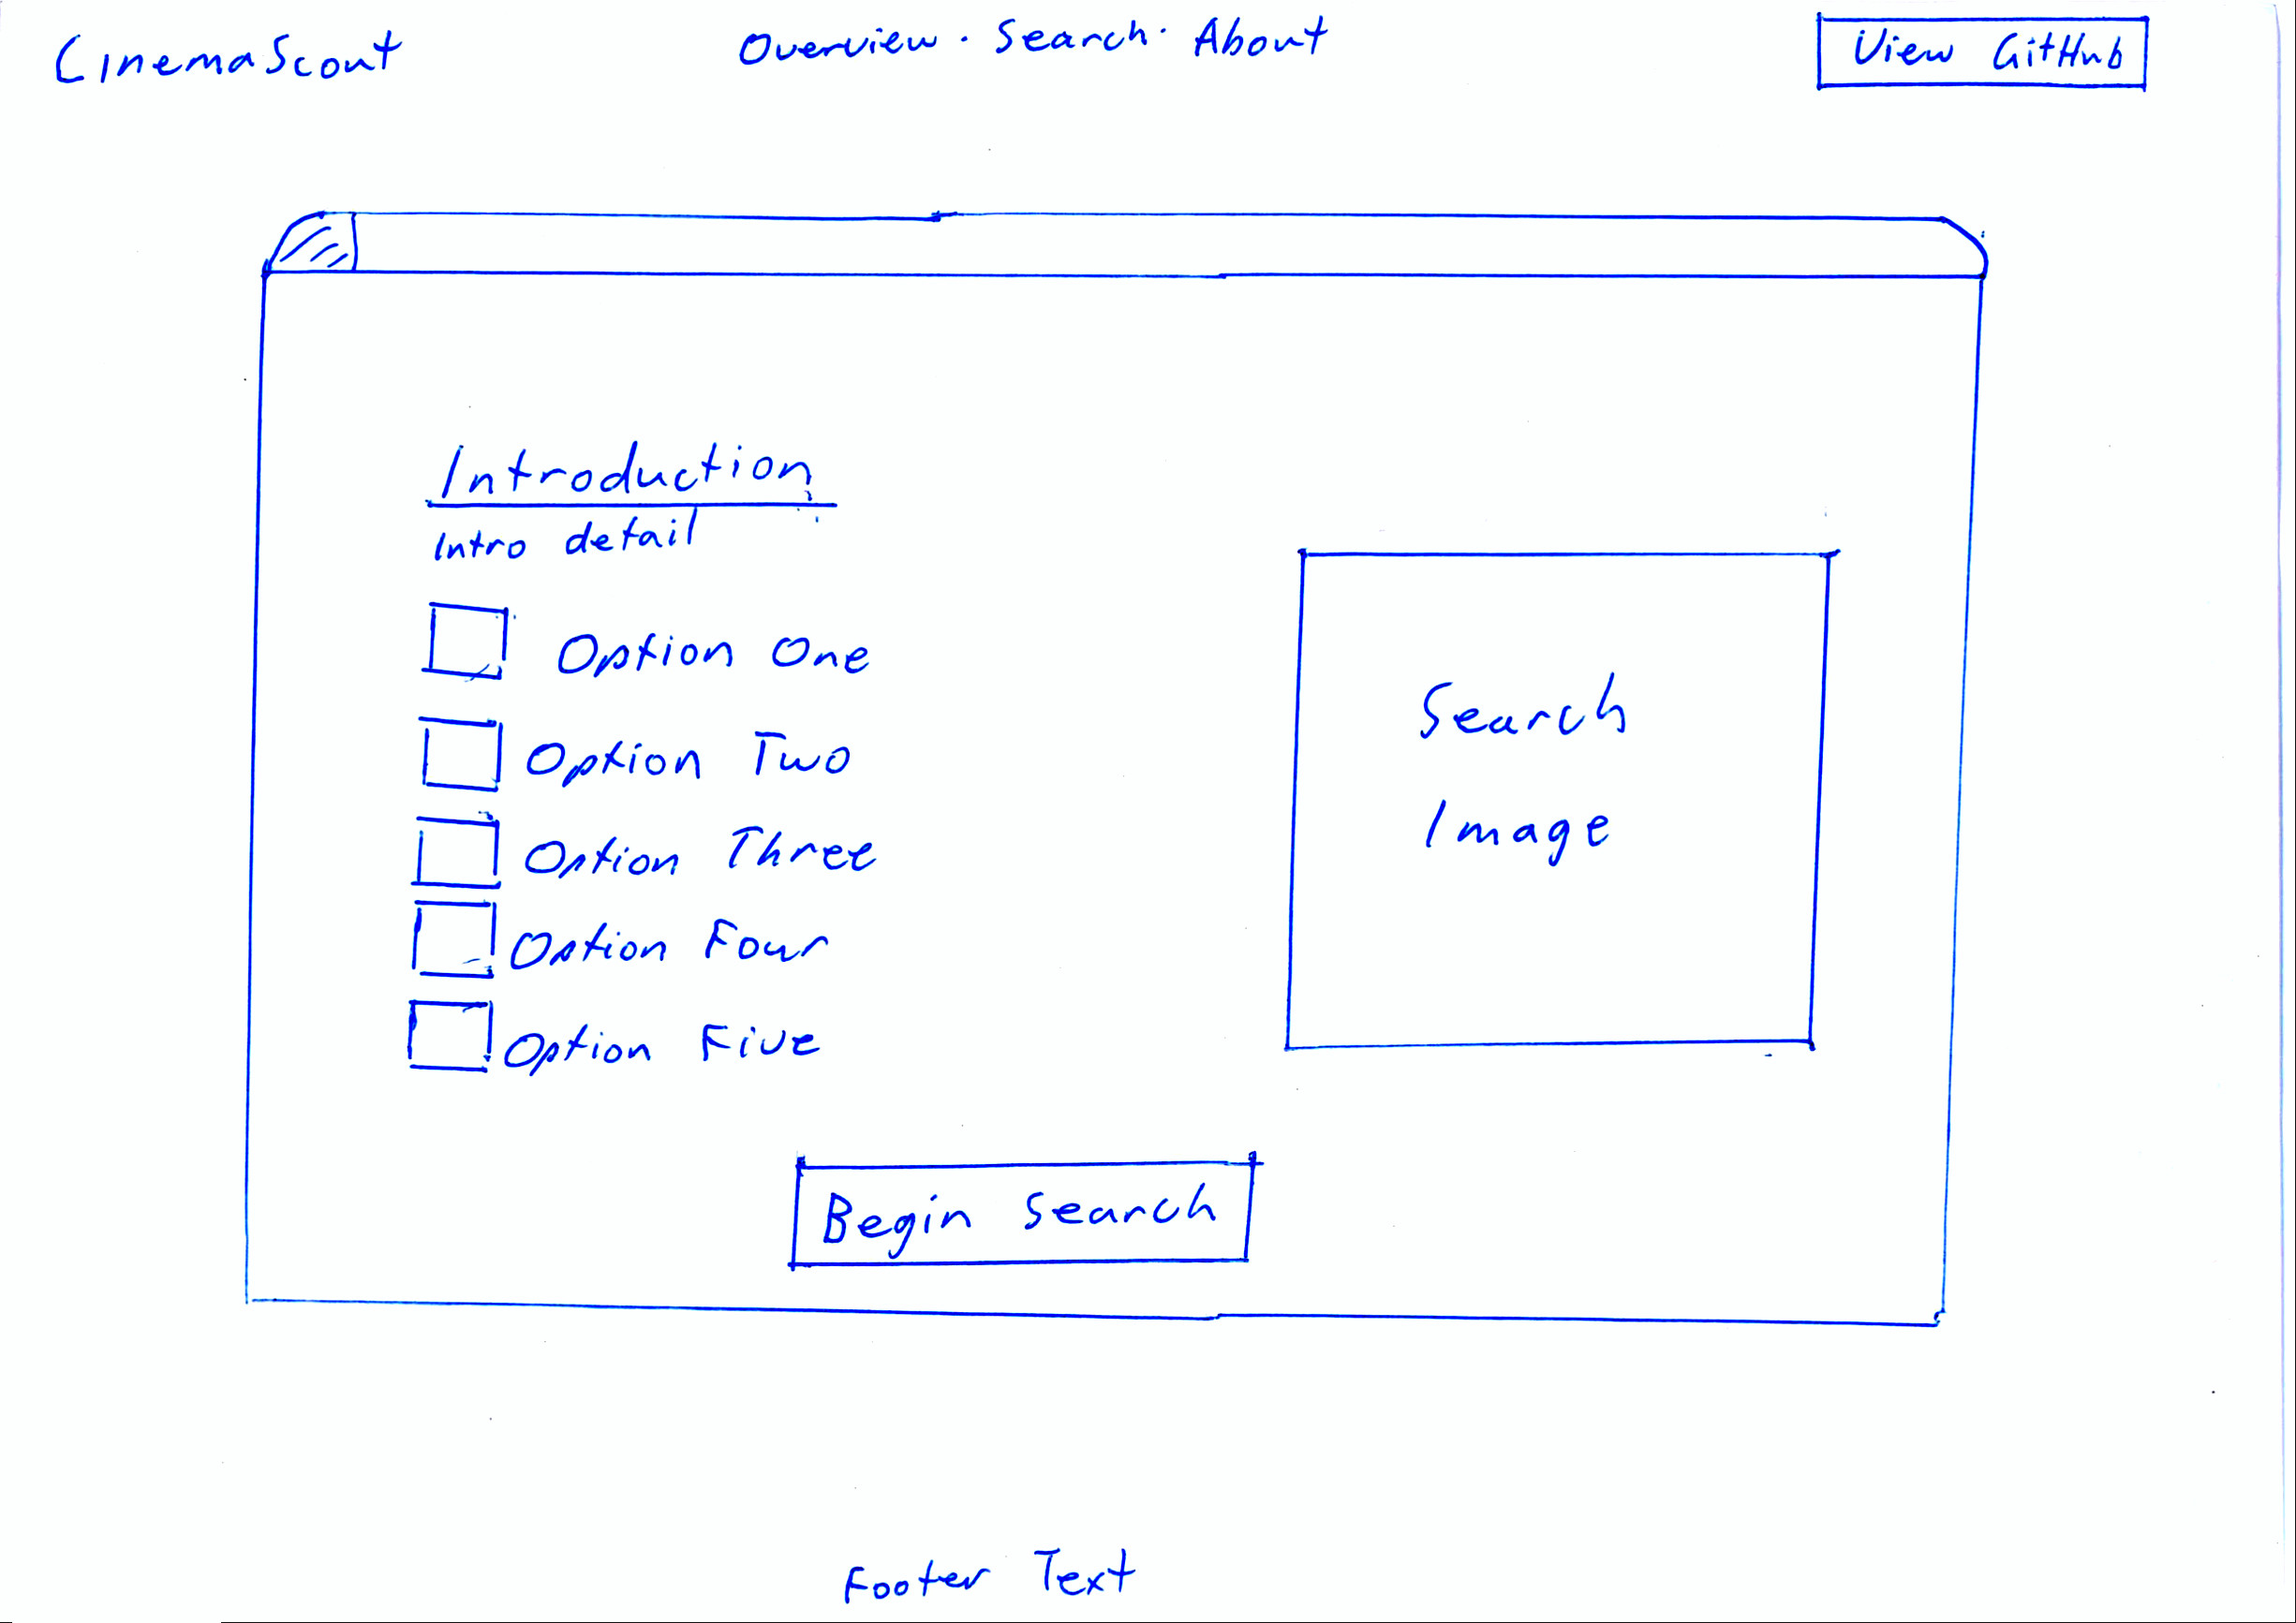
\includegraphics[width=\columnwidth]{res/search_begin.jpg}
\caption{Rough sketch of the initialise search state of the search page.}
\end{figure}
\begin{figure}[H]
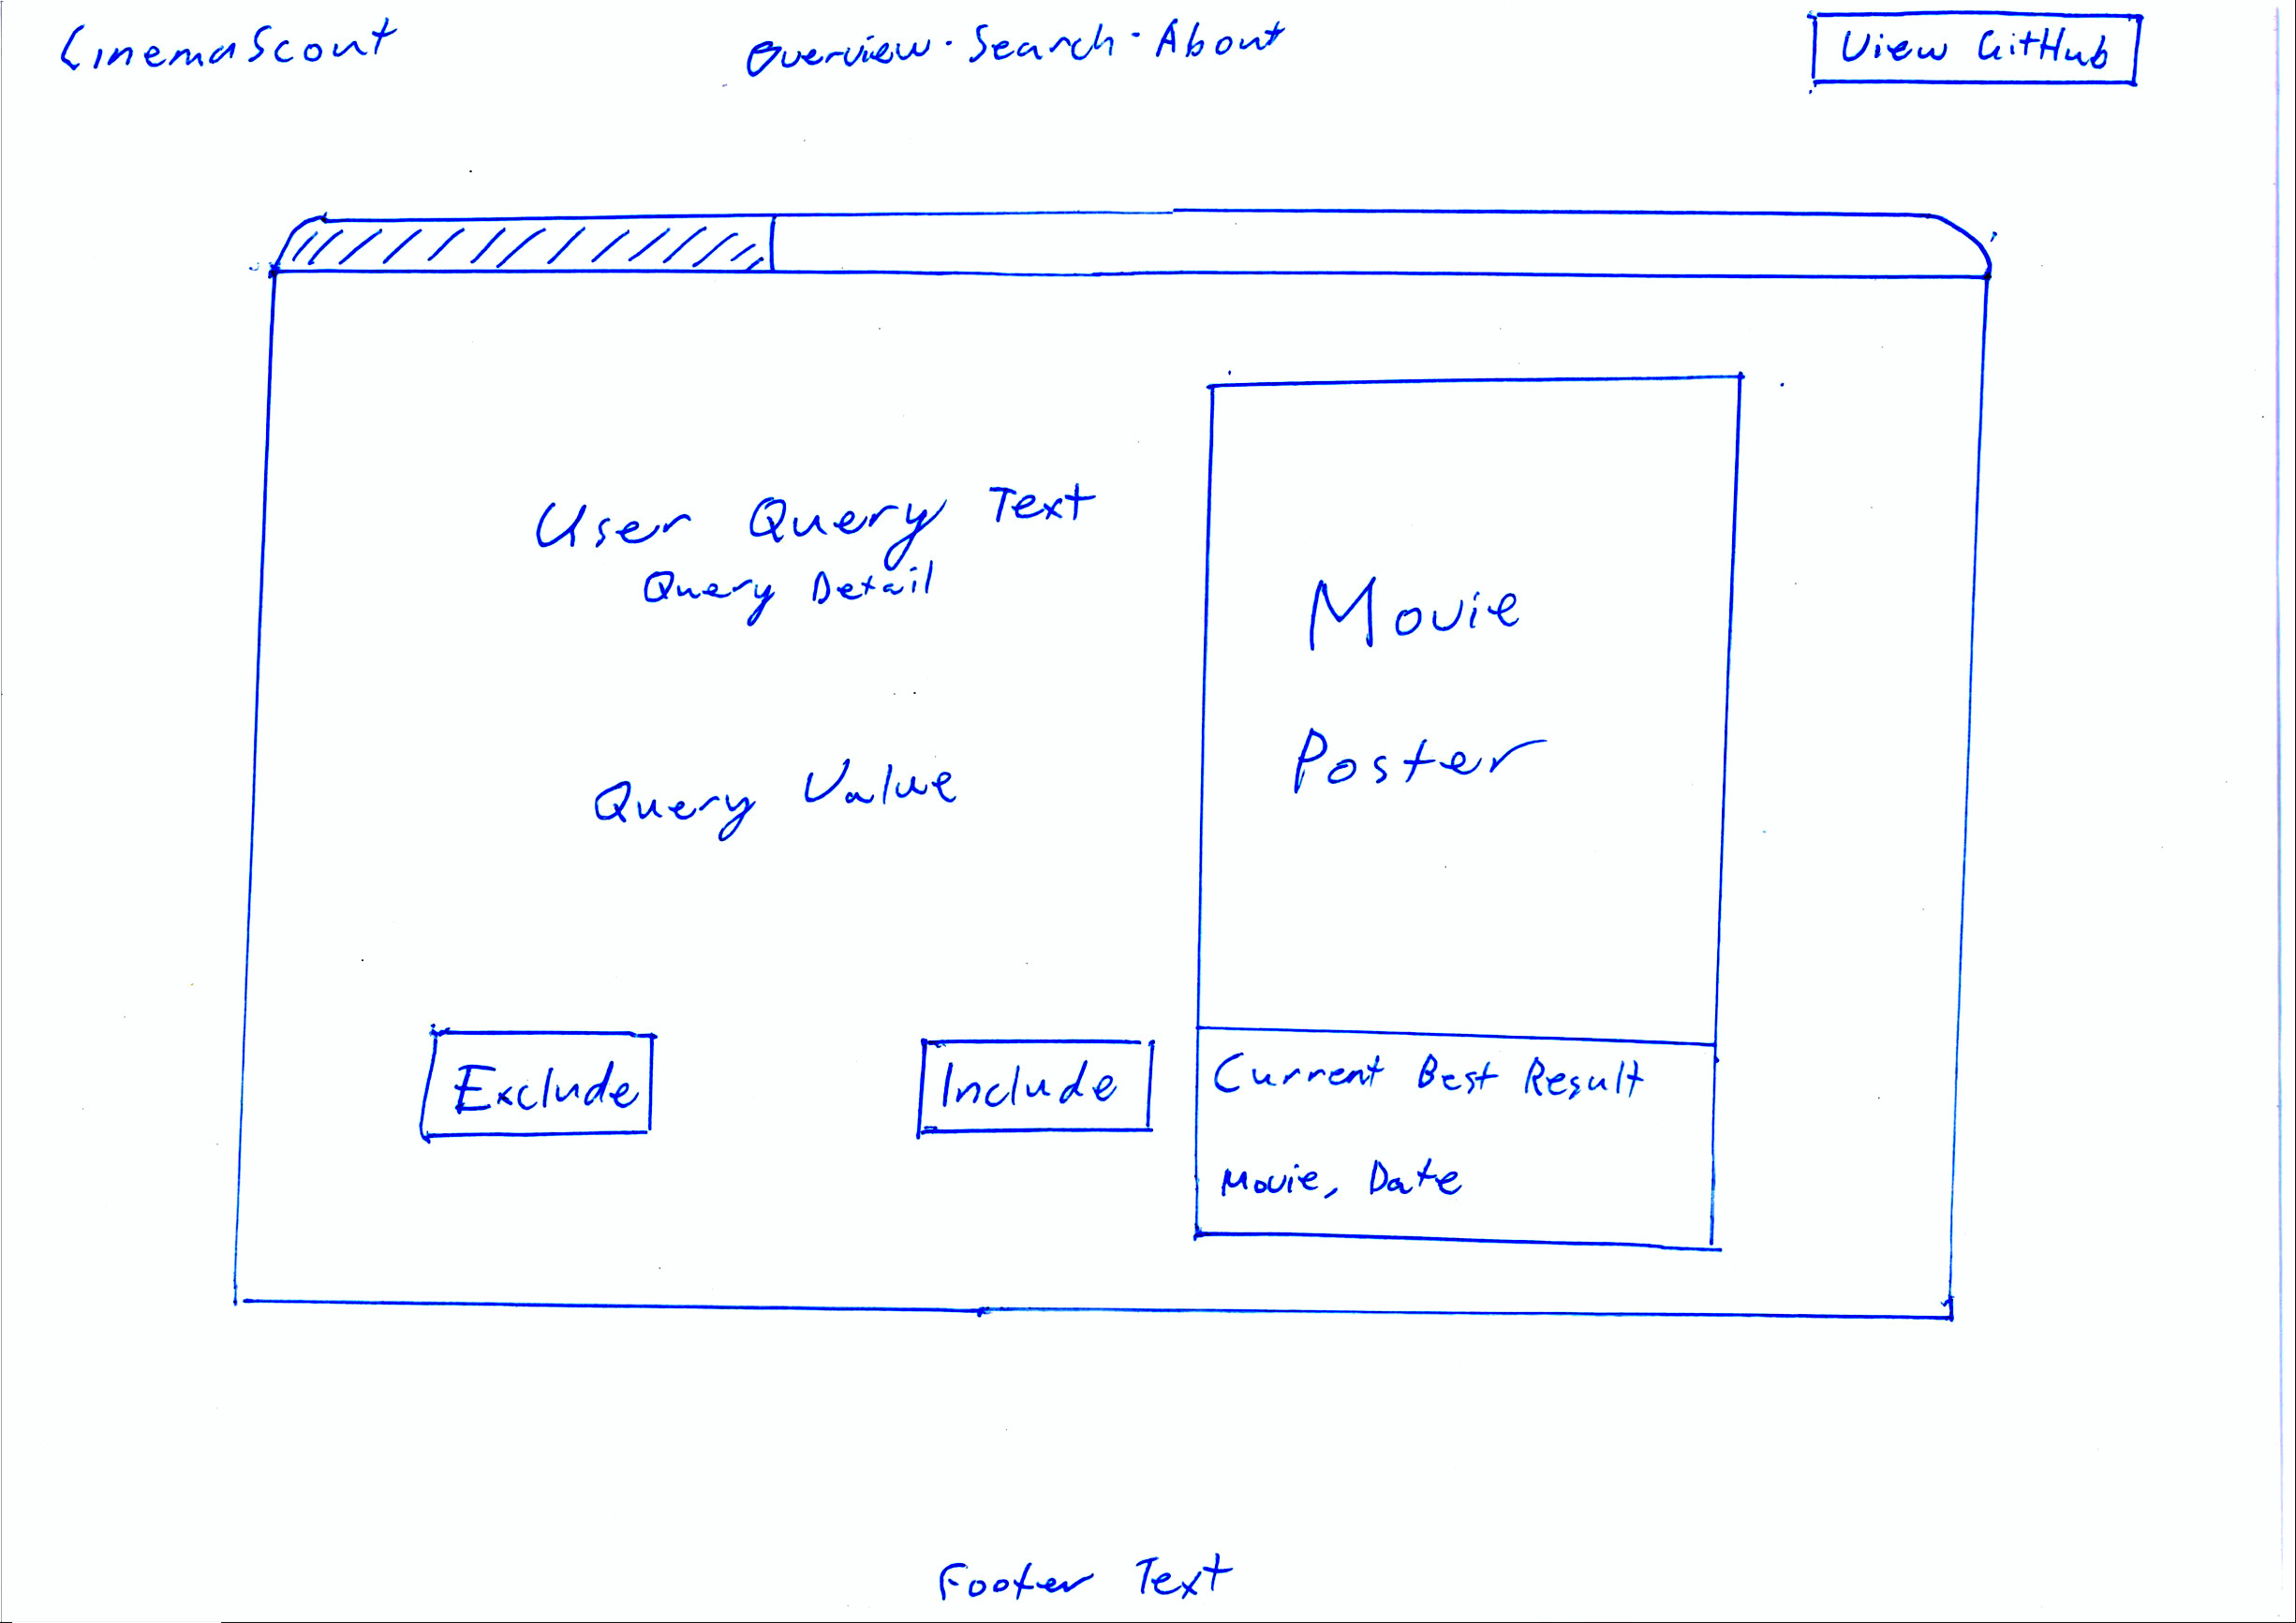
\includegraphics[width=\columnwidth]{res/search_next.jpg}
\caption{Rough sketch of the in progress state of the search page.}
\end{figure}
\subsection{About Page}
\begin{figure}[H]
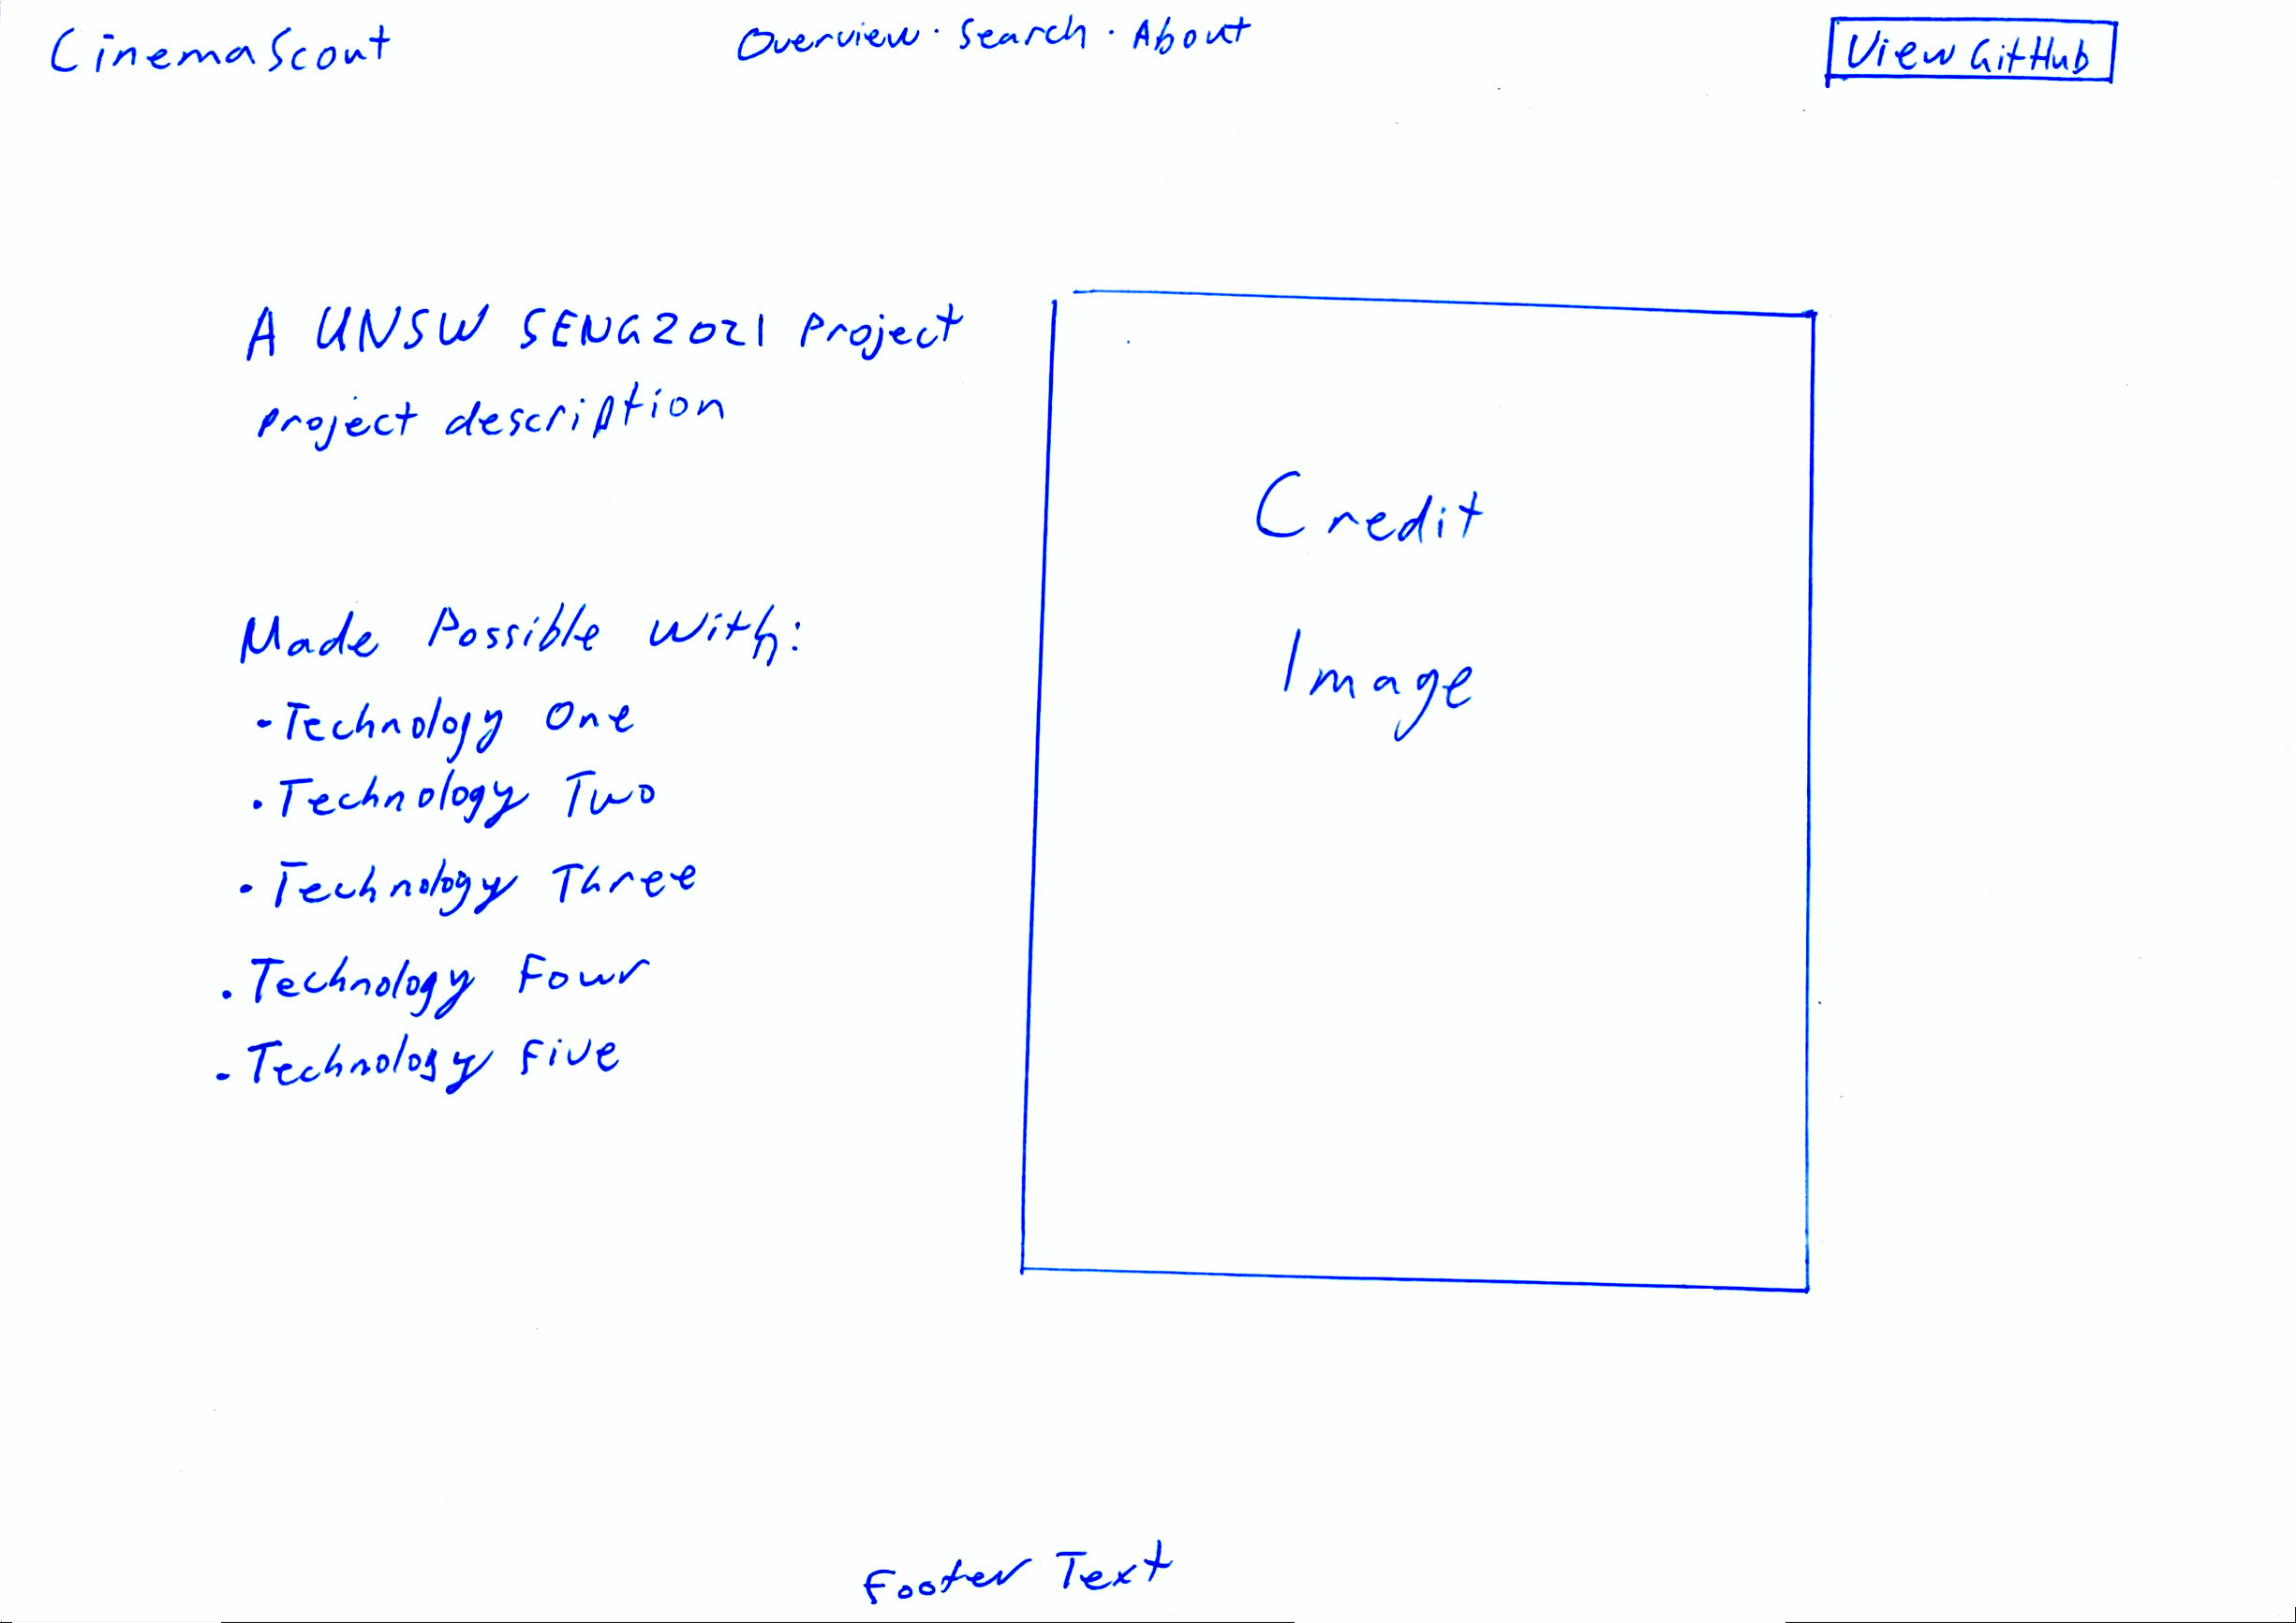
\includegraphics[width=\columnwidth]{res/credits.jpg}
\caption{Rough sketch of the about page.}
\end{figure}
\subsection{Storyboard Composite}
\begin{figure}[H]
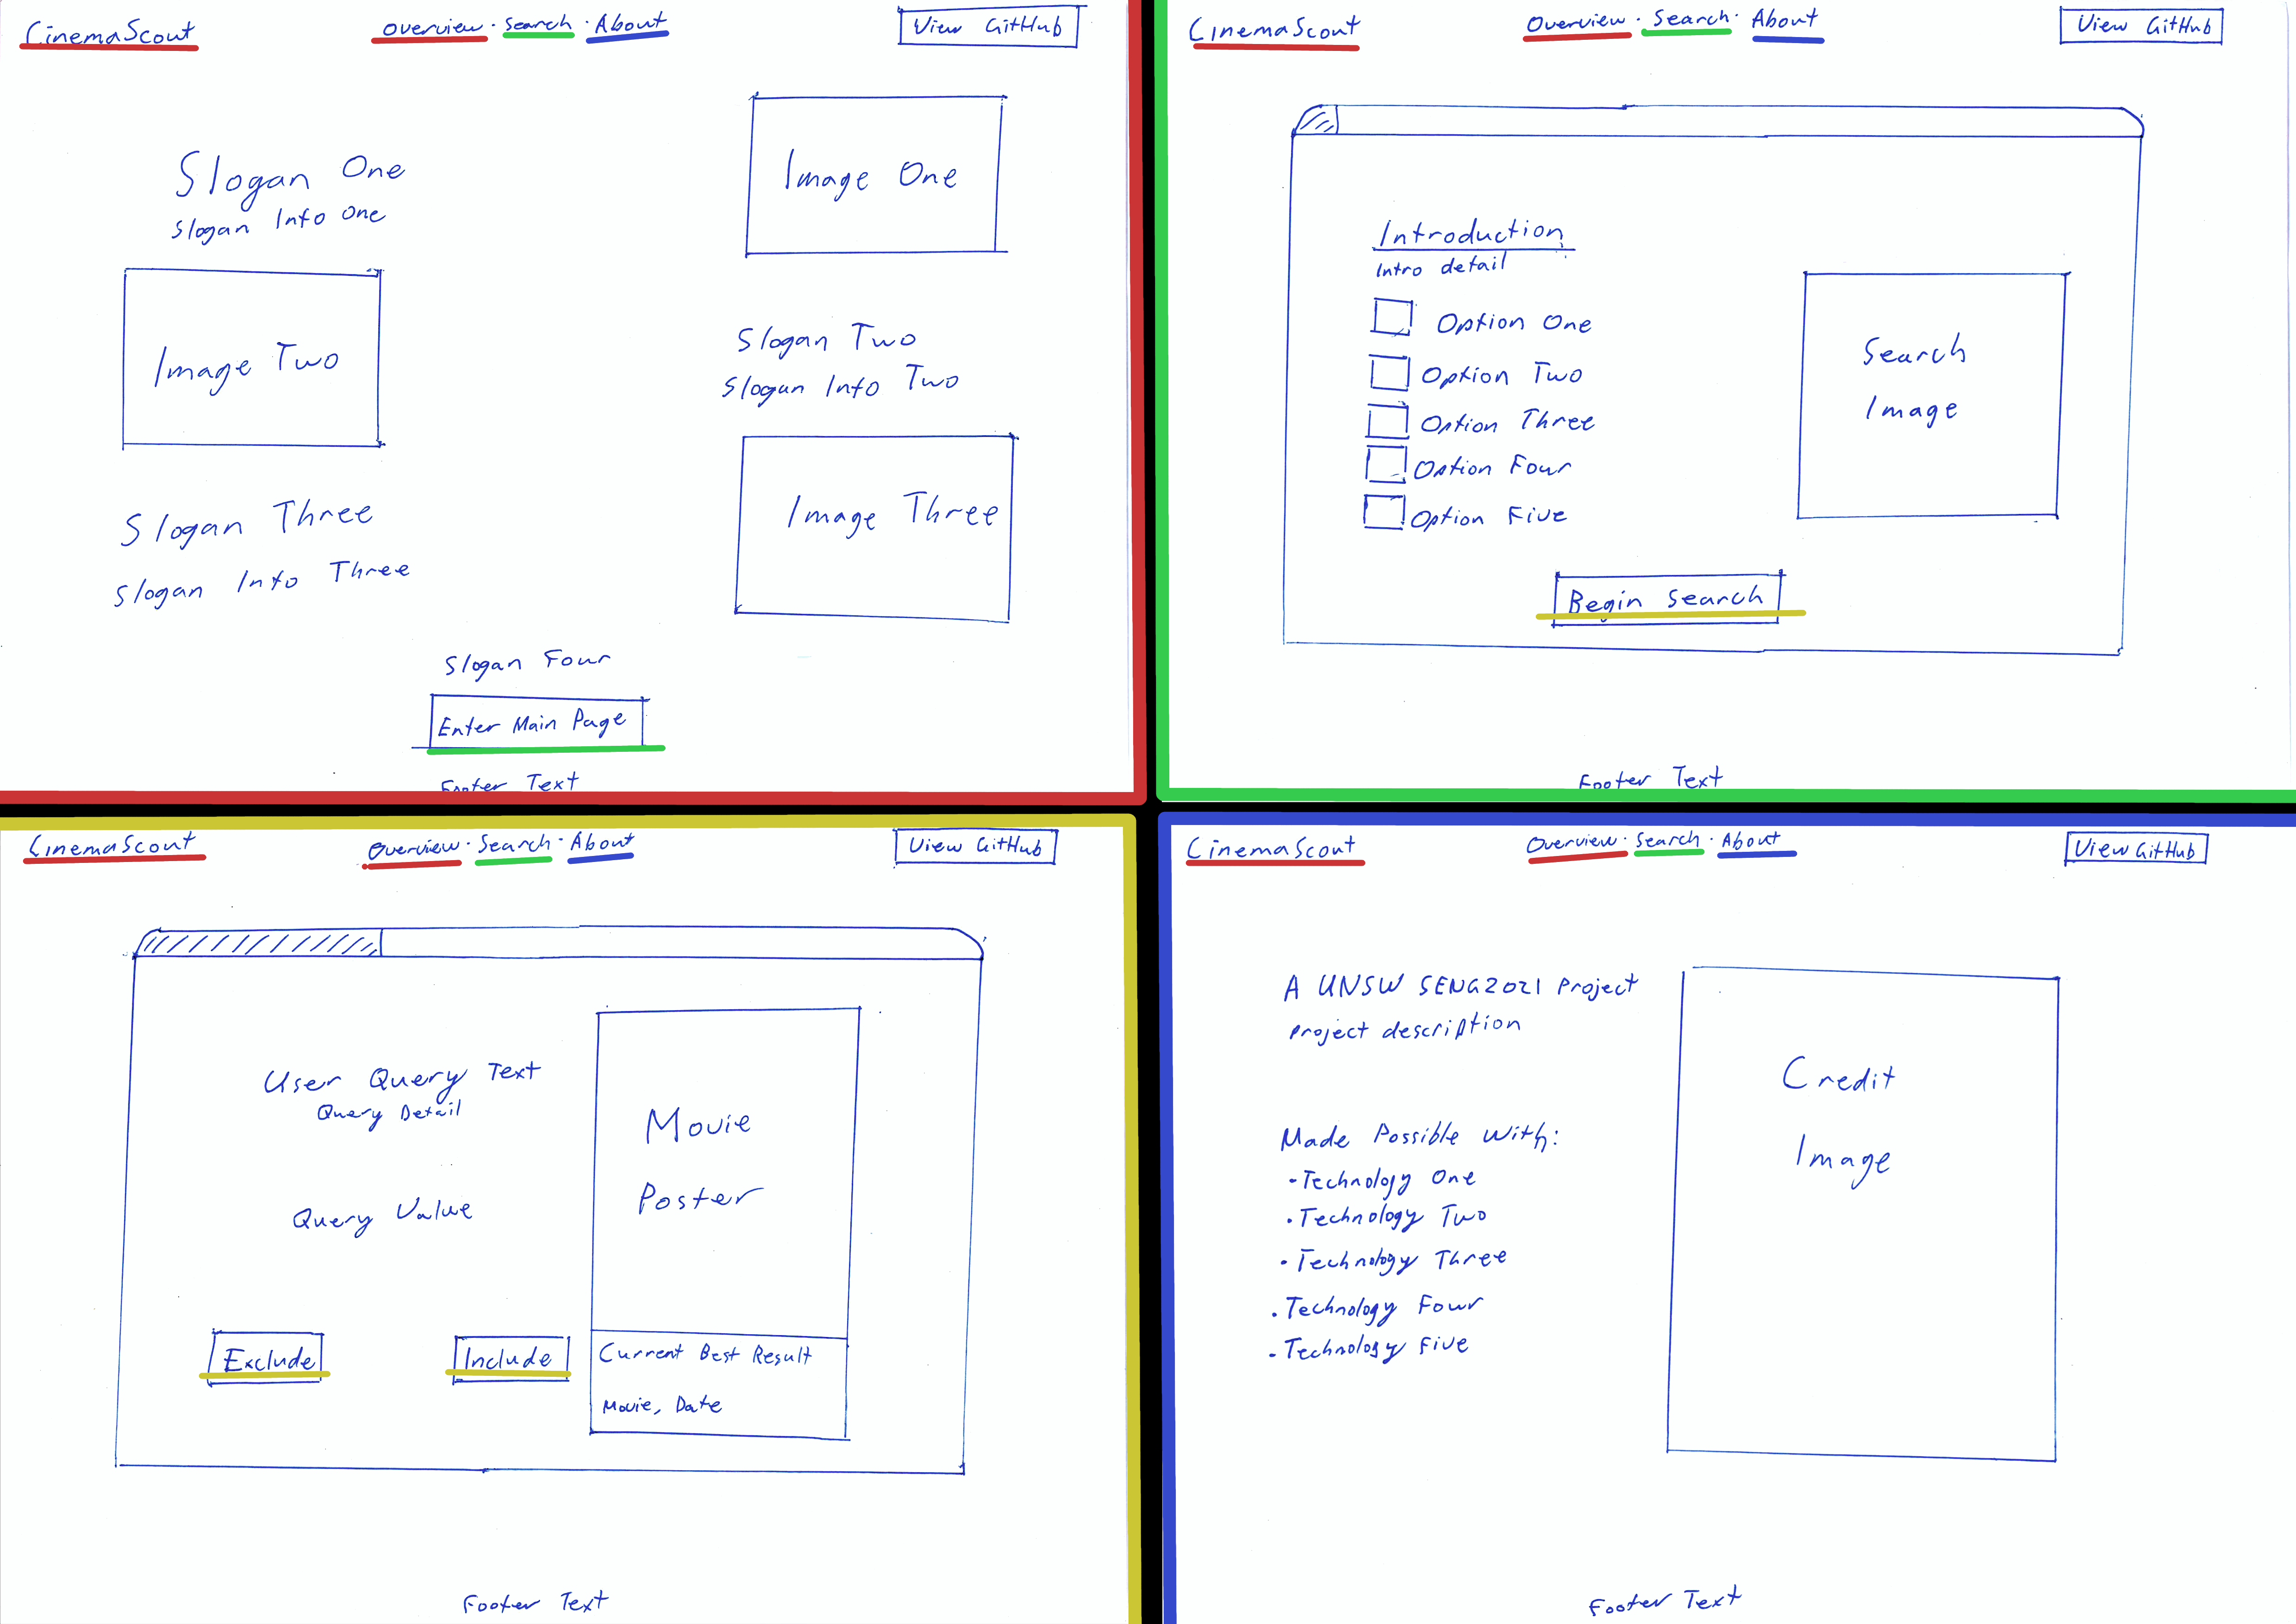
\includegraphics[width=\columnwidth]{res/arrows.png}
\caption{Storyboard sketch of all previous figures.}
\end{figure}

\section{High-Fiedelity Prototype}
The following images are a work in progress and do not represent the final
design of the product. All images were captured at a resolution of 1920 x
1080 using a default Chromium browser on Arch Linux.
\subsection{Landing Page}
\begin{figure}[H]
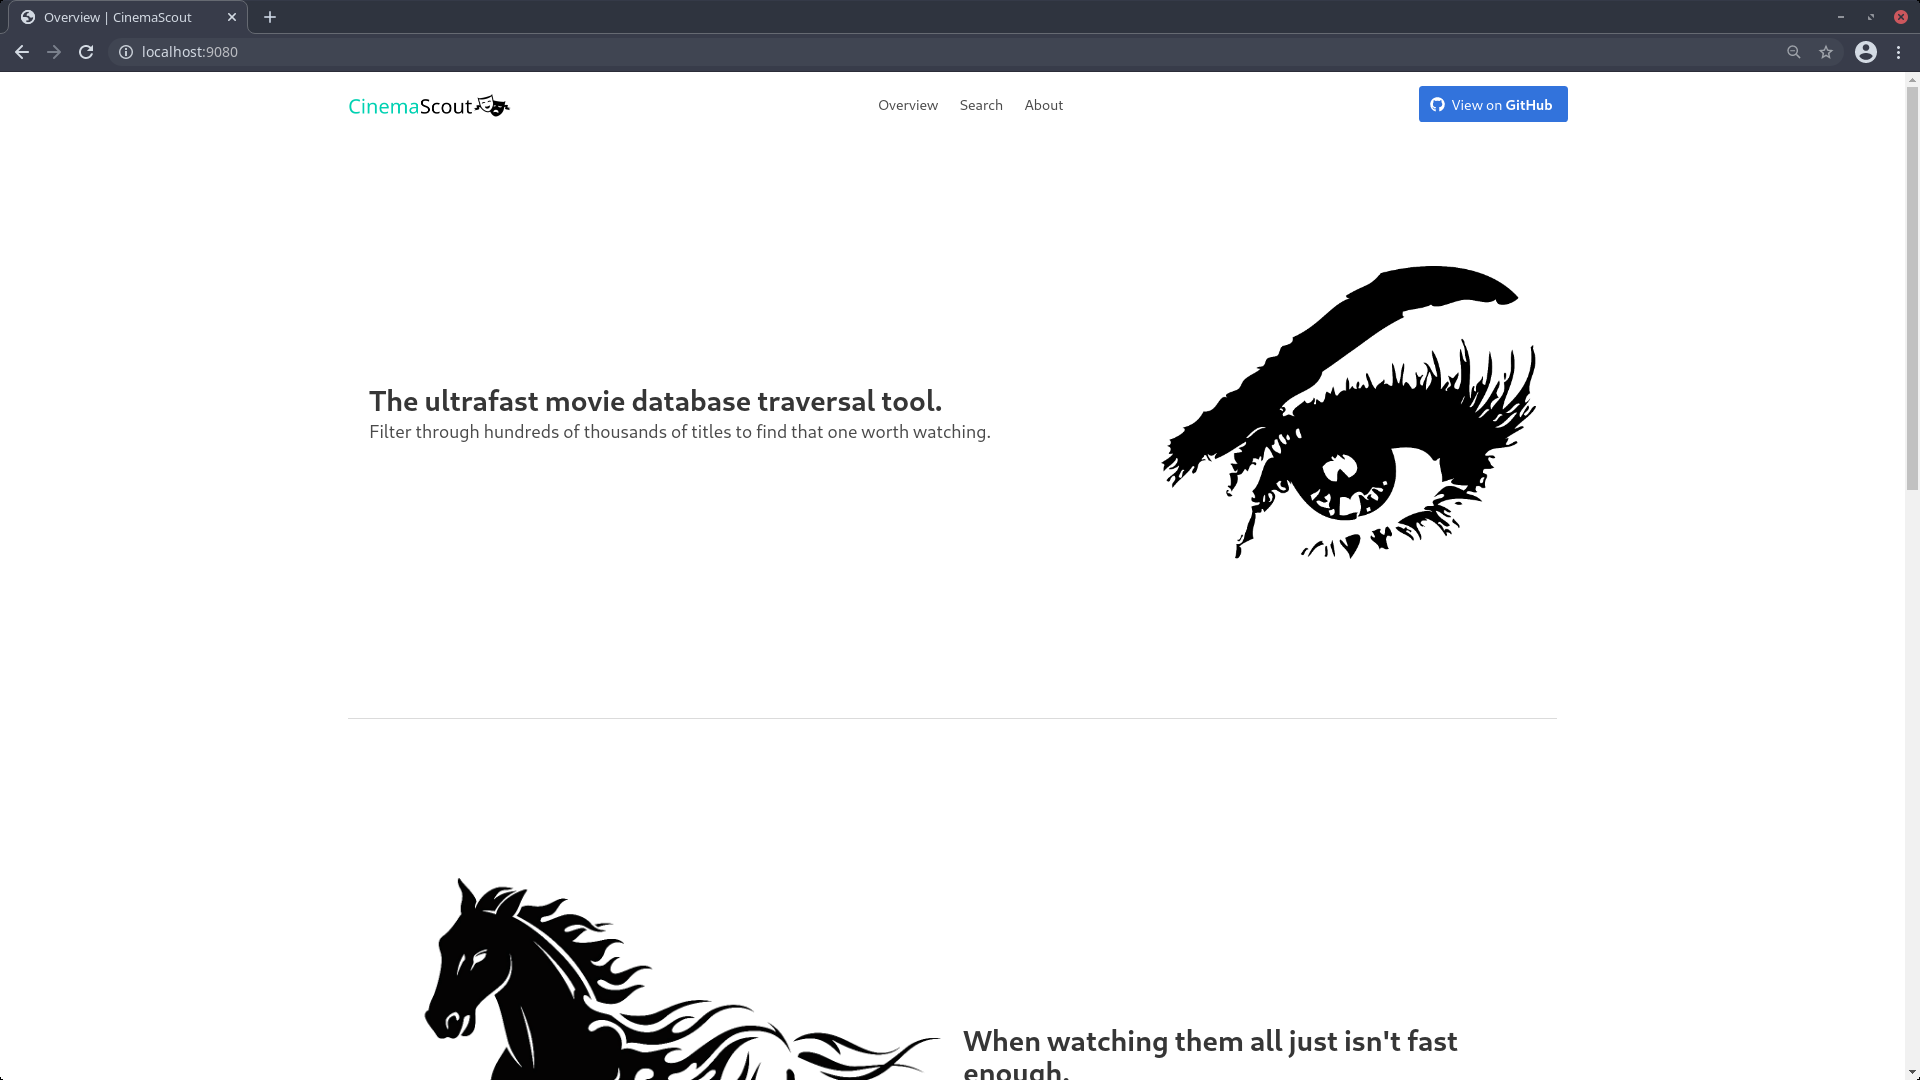
\includegraphics[width=\columnwidth]{res/landing_1.png}
\caption{Upper portion of the landing page.}
\end{figure}
\begin{figure}[H]
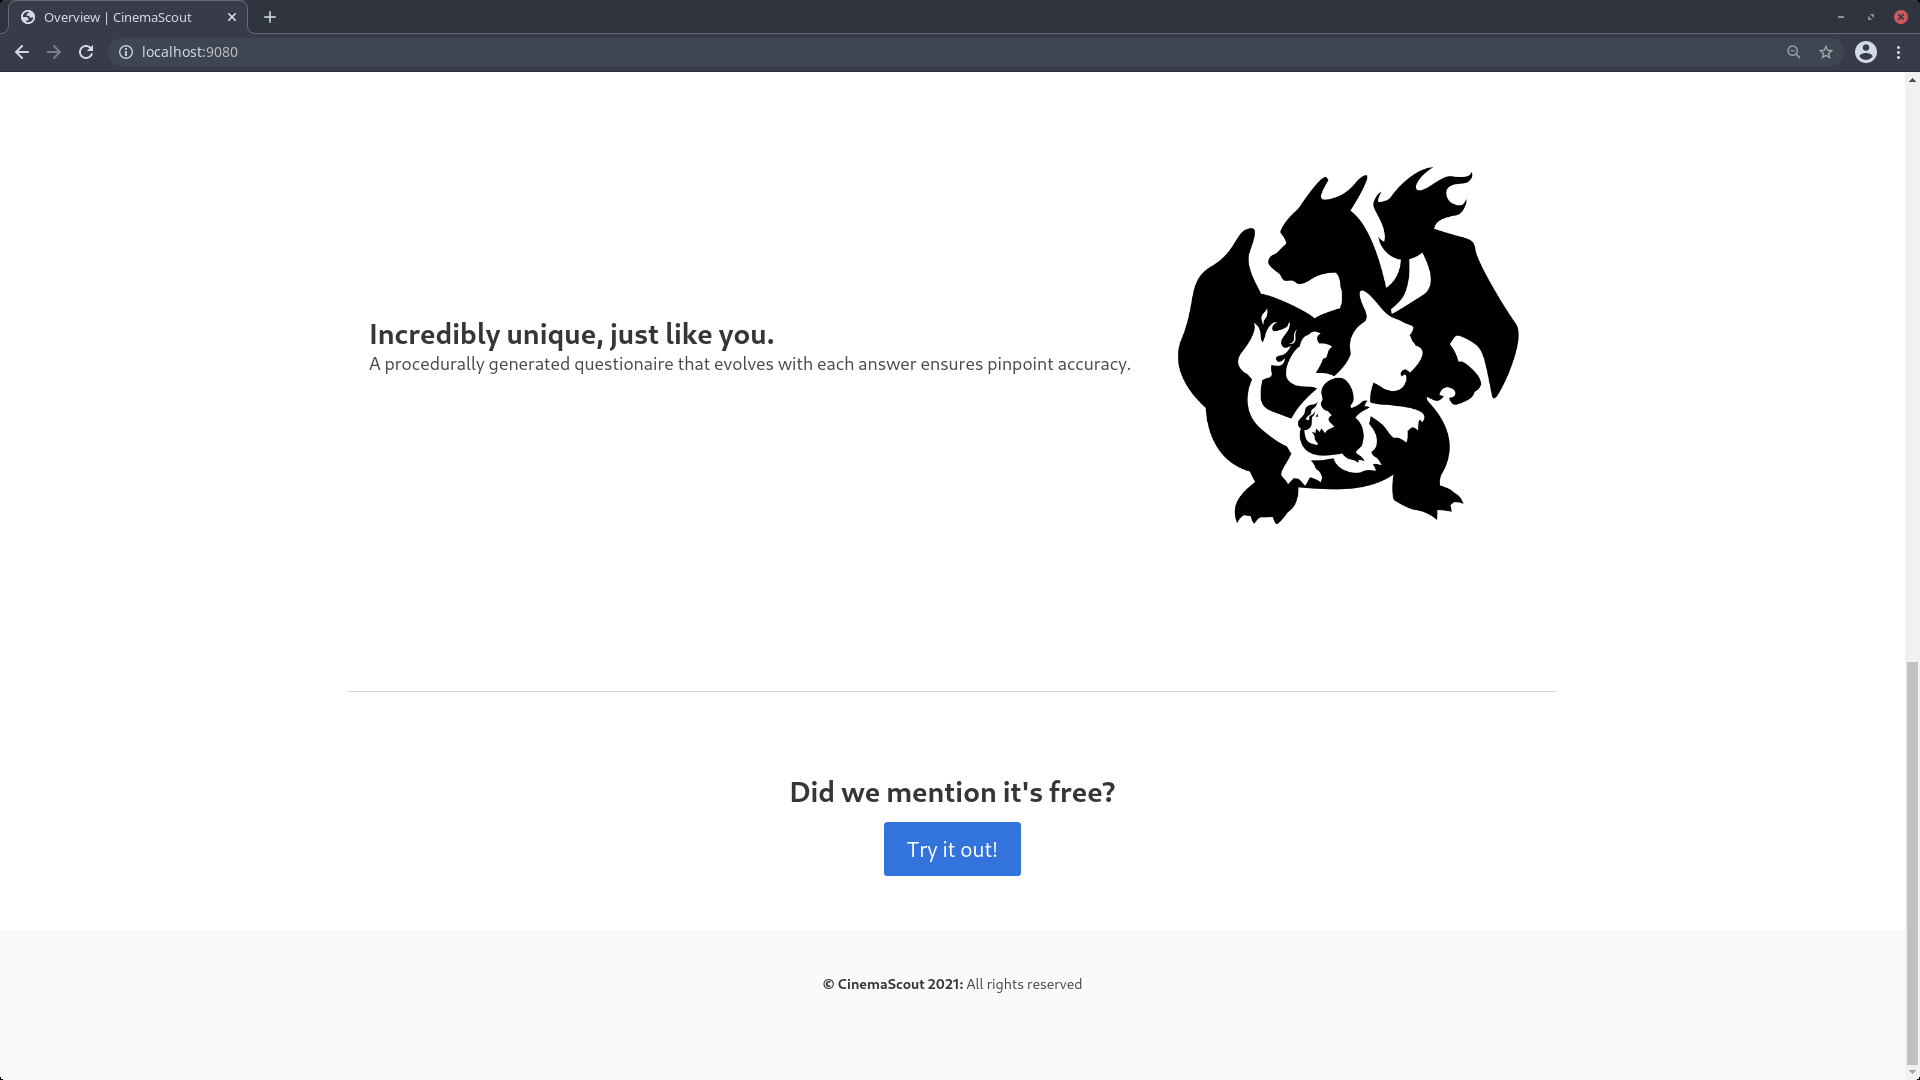
\includegraphics[width=\columnwidth]{res/landing_2.png}
\caption{Lower portion of the landing page.}
\end{figure}
\subsection{Search Page}
\begin{figure}[H]
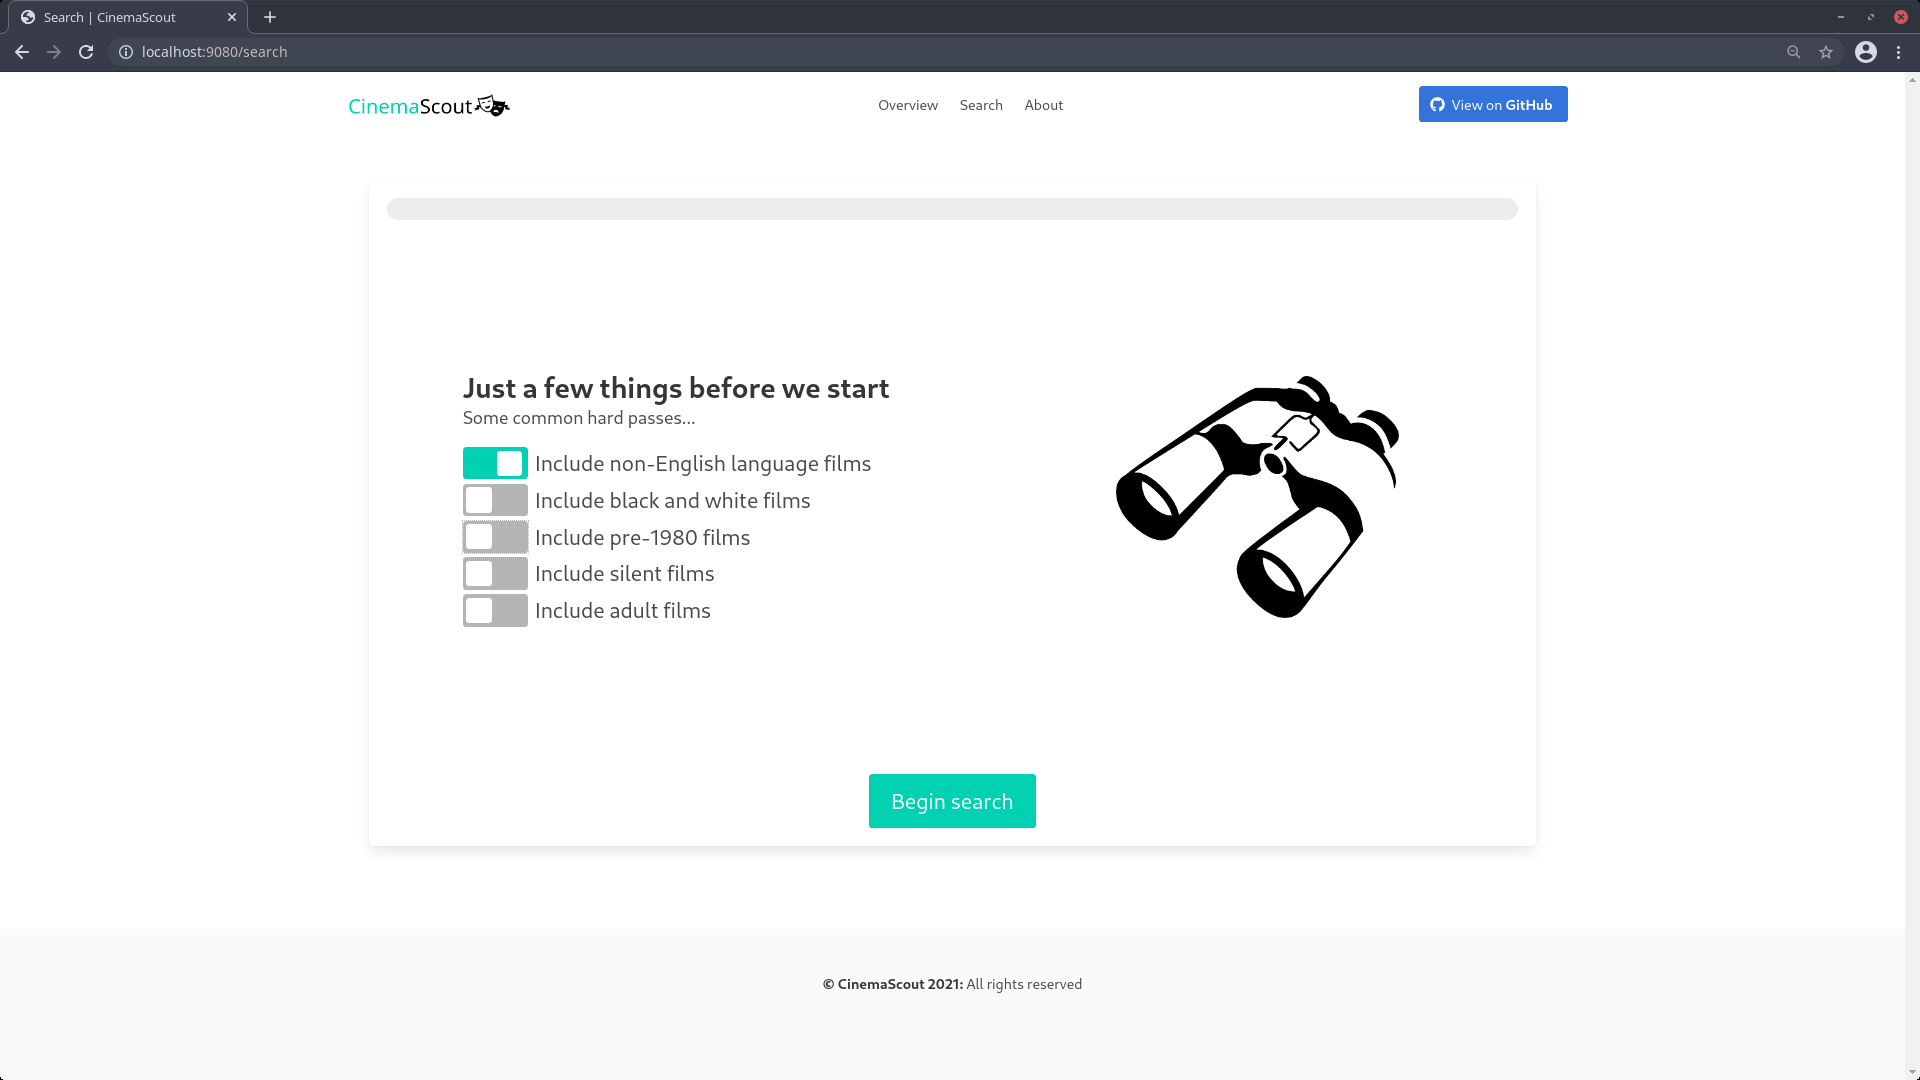
\includegraphics[width=\columnwidth]{res/search_1.png}
\caption{Initialise search state of the search page.}
\end{figure}
\begin{figure}[H]
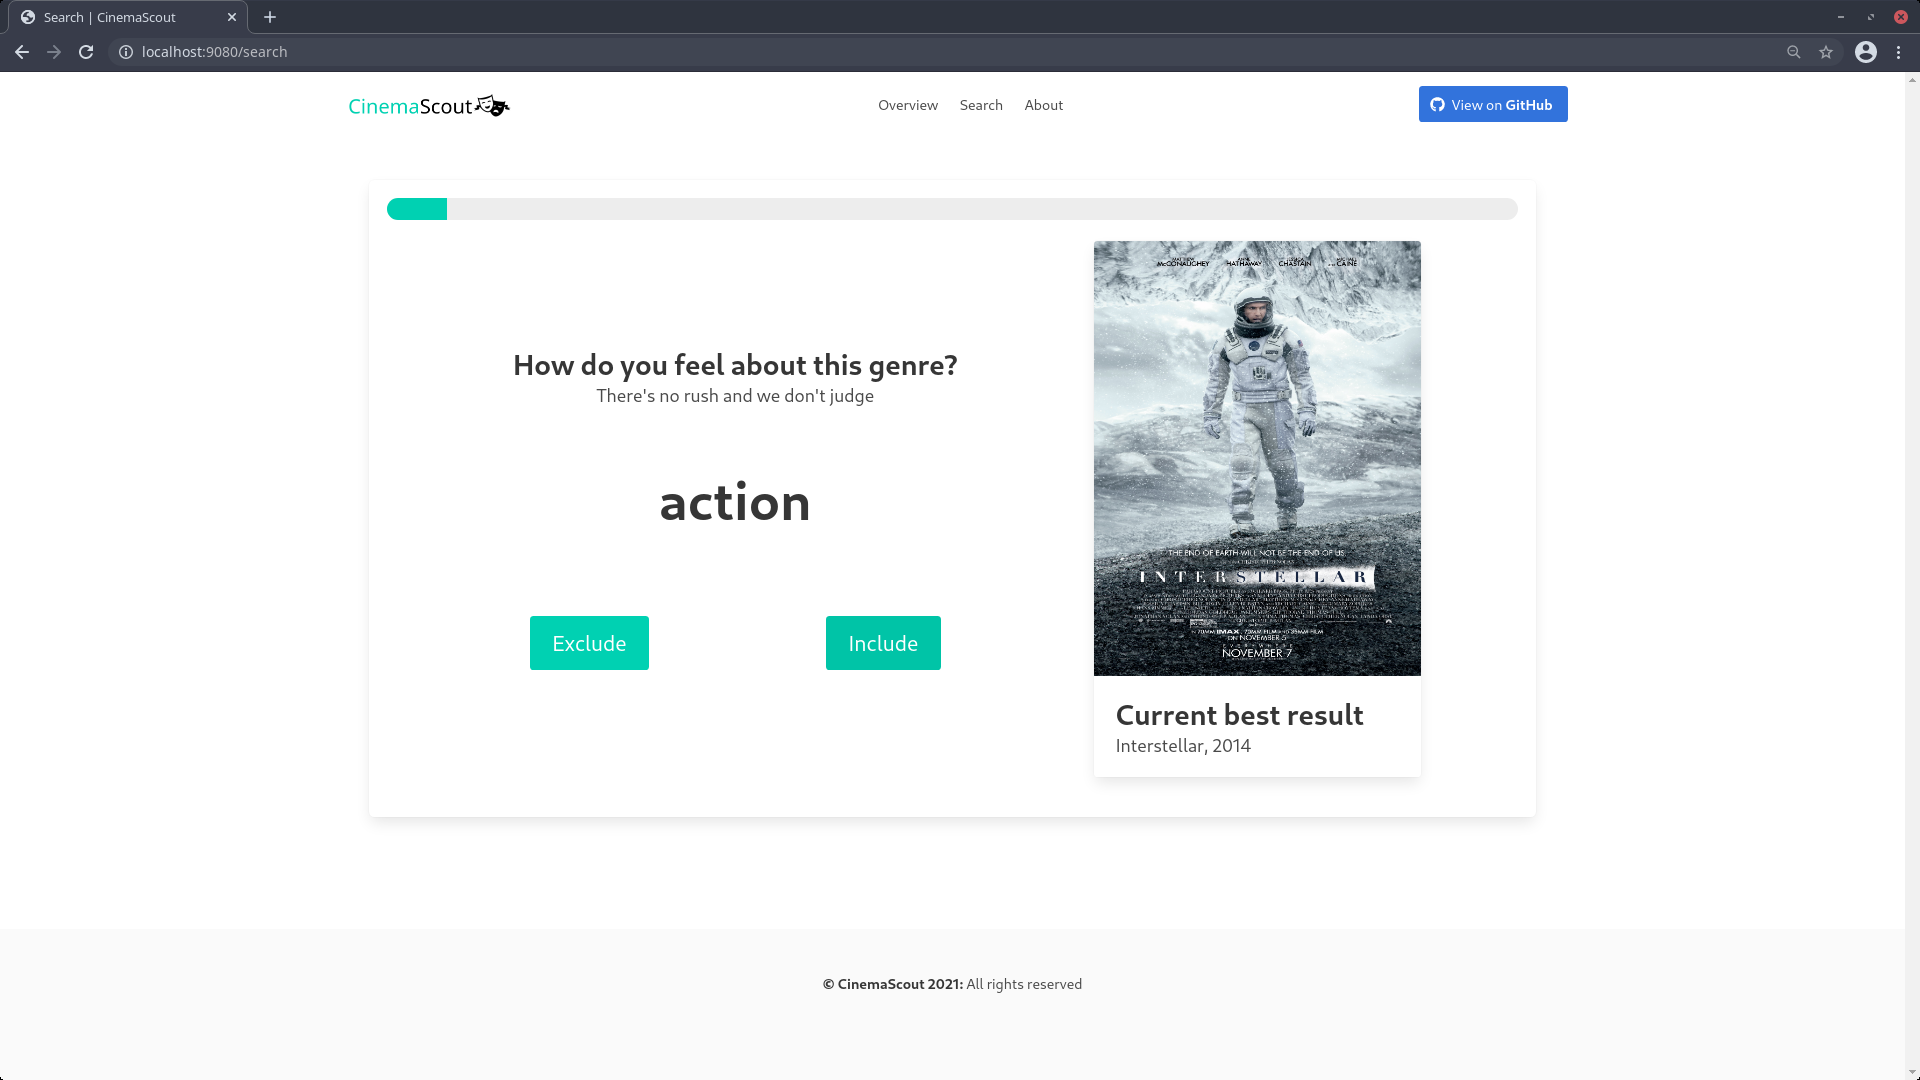
\includegraphics[width=\columnwidth]{res/search_2.png}
\caption{Search in progress state of the search page.}
\end{figure}
\subsection{About Page}
\begin{figure}[H]
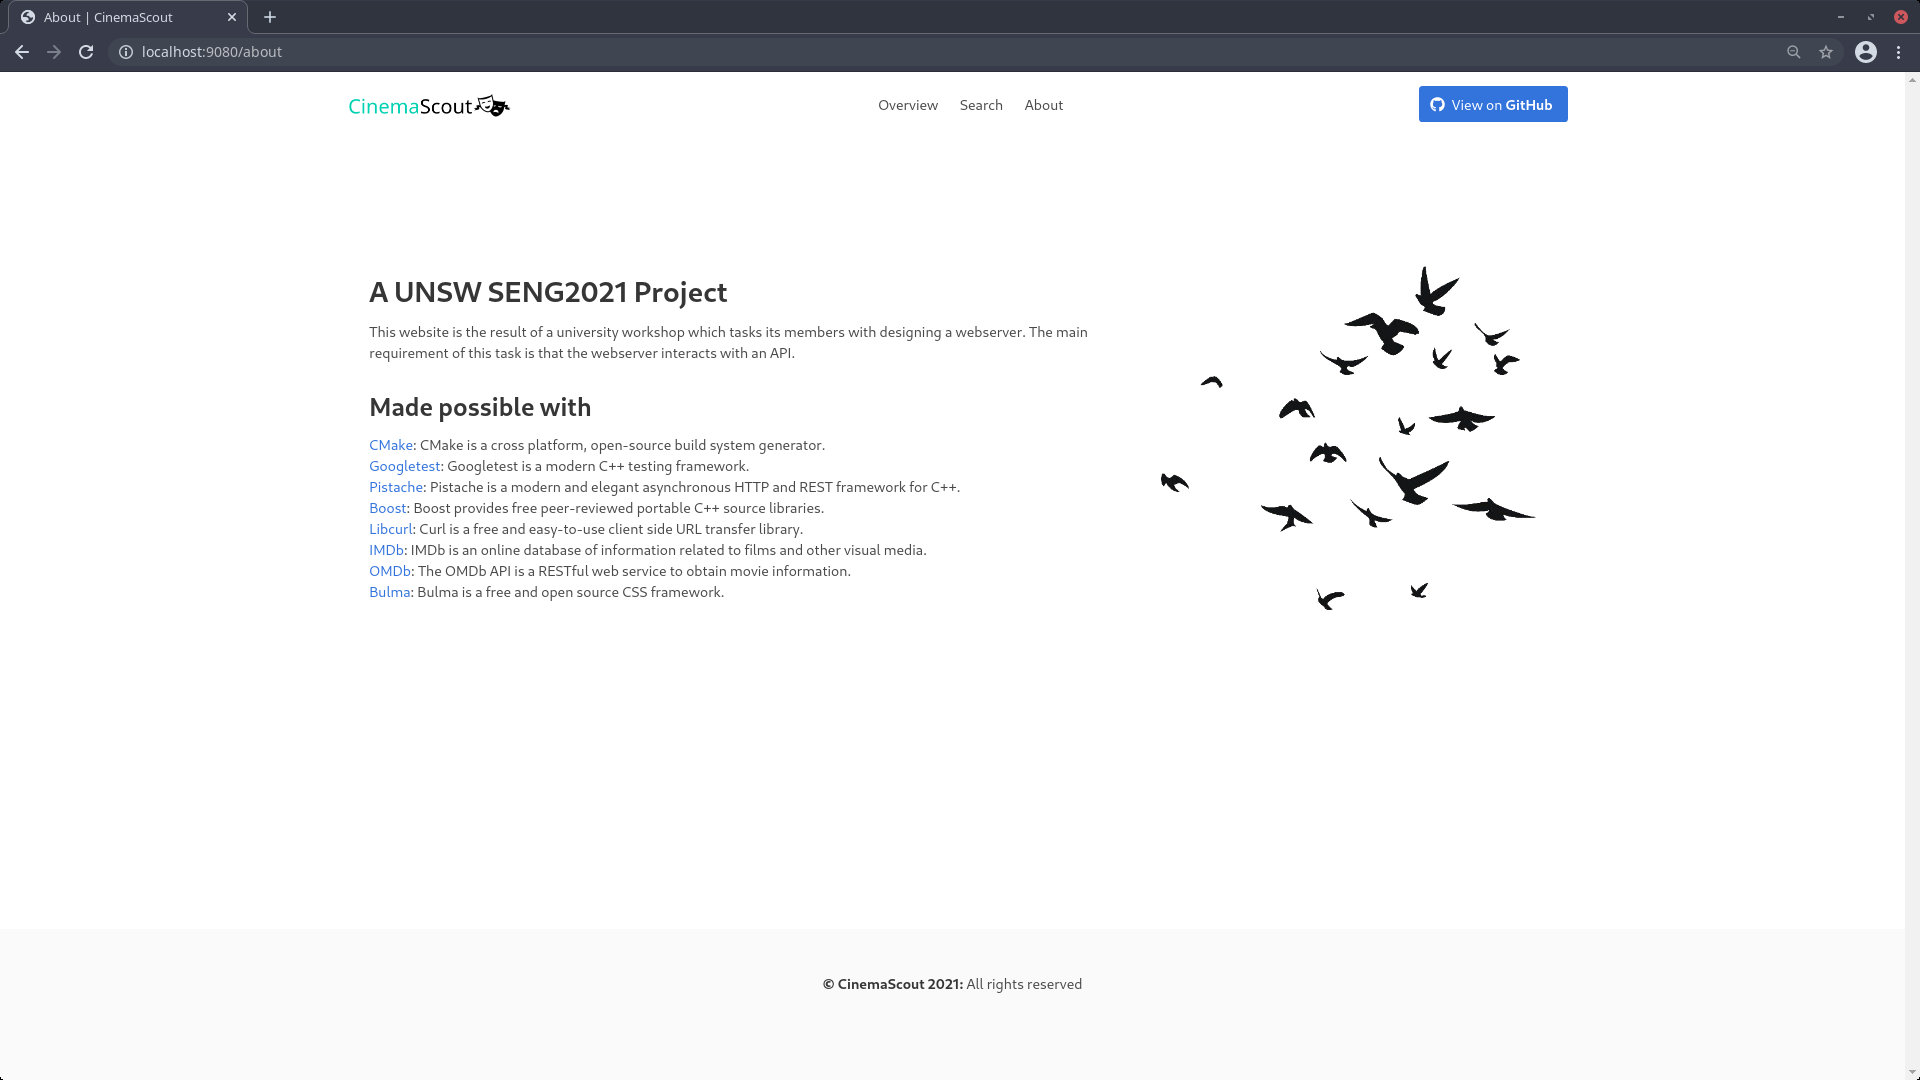
\includegraphics[width=\columnwidth]{res/about.png}
\caption{Entire portion of the about page.}
\end{figure}

\end{document}
